\documentclass[11pt]{article}
\usepackage[T1,T2A]{fontenc}
\usepackage[utf8]{inputenc}
\usepackage[english,russian]{babel}
\usepackage{graphicx}
\usepackage{amsmath}
\graphicspath {{img/}}

\title{\textbf{Лабораторная работа №6\\<<Помехоустойчивое кодирование. Код Хэмминга>>}}
\author{Перепелица А.А., ККСО-01-19}
\date{Москва, 2022 г.}
\addtolength{\topmargin}{-3cm}
\addtolength{\textheight}{3cm}
\begin{document}
\maketitle
\thispagestyle{empty}
\textbf{Цель работы:}  ознакомление с принципами помехоустойчивого кодирования и приобретение практических навыков моделирования работы кодеров и декодеров. 

\section{Задание №1: формирование бита чётности}
\subsection{Исходные данные для задания}
\includegraphics[width=1\linewidth]{img/sheet1.png}
\begin{center}
    Таблица 1 - Исходные данные для задания №1
\end{center}
\subsection{Формирование бита чётности}


\newpage
\section{Задание №2: Исследование помехоустойчивого кода с формированием бита чётности}
\subsection{Исходные данные для задания}
\includegraphics[width=1\linewidth]{img/sheet2.png}
\begin{center}
    Таблица 2 - Исходные данные для задания №2
\end{center}

\subsection{Схема для моделирования процесса передачи информации по каналу связи}
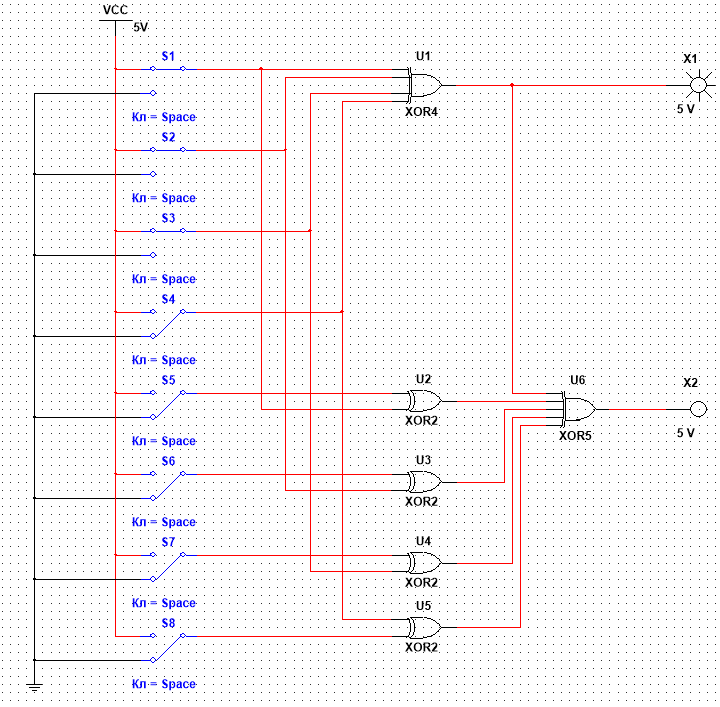
\includegraphics[width=1\linewidth]{img/scheme1.png}
\begin{center}
    Рис. 1 - Схема для исследования кода с формированием бита чётности
\end{center}

\subsection{Результаты расчетов}
\begin{center}
    \includegraphics[width=1\linewidth]{img/sheet3.png}
        Таблица 3 - Полученные результаты при заданных значениях.
\end{center}


\newpage
\section{Задание №3: Исправление ошибки с помощью кода Хэмминга}
\subsection{Исходные данные для задания}
\begin{center}
    \includegraphics[width=1\linewidth]{img/sheet3.png}
        Таблица 4 - Исходные данные для задания №3.
\end{center}

\subsection{Процесс вычисления искажённого бита}


\newpage
\section{Задание №4: Моделирование работы кода Хэмминга}
\subsection{Исходные данные для задания}
Исходные данные приведены в таблице 3.
\subsection{Схема для исследования работы кода Хэмминга}
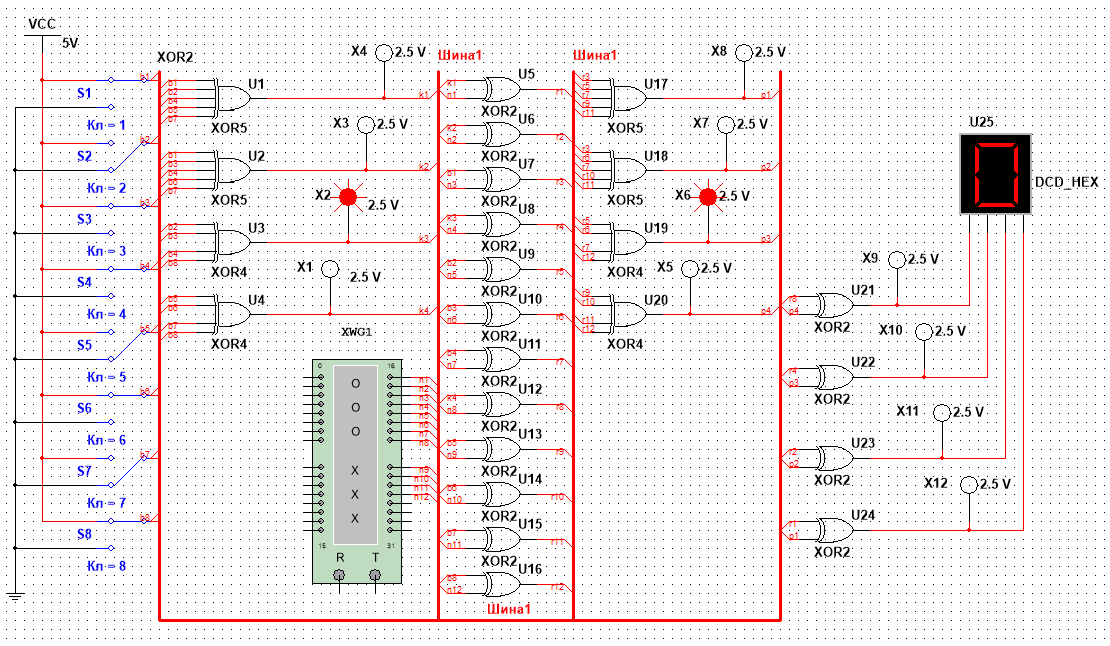
\includegraphics[width=1\linewidth]{img/scheme2.png}
\begin{center}
        Рис 2 - Схема моделирования работы кода Хэмминга в системе передачи информации.
\end{center}

\subsection{Результаты расчётов}

\textbf{Вывод:} В ходе выполнения лабораторной работы мы изучили устройства фазового преобразования сигналов, их работу. Также получили практические навыки, научились моделировать эти устройства.


\end{document}